\documentclass[12pt]{exam}
\usepackage[top=1in, bottom=1in, left=.45in, right=.45in]{geometry}
\usepackage{amsmath,amsthm,amssymb,amstext}
\usepackage{enumerate,enumitem}
\usepackage{tikz,float,graphicx}
\usepackage{microtype}
\usepackage{bm,tikz}
\usepackage{multicol}
\usepackage[framemethod=tikz]{mdframed}
\usetikzlibrary{calc}

\newcommand{\course}{MTH 234 Summer 2021}
\newcommand{\qdate}{The Dot Product} %PUT DATE HERE
\newcommand{\quiz}{Group Work} 

\newcommand{\gen}[1]{\left\langle #1 \right\rangle}
\newcommand{\ba}{\bm{a}}
\newcommand{\bb}{\bm{b}}
\newcommand{\bc}{\bm{c}}

\printanswers

\newtheorem*{definition}{Definition}
\surroundwithmdframed[]{definition}
\newtheorem*{theorem}{Theorem}
\surroundwithmdframed[]{theorem}

%%%%%%%%%%%%%%%%%%%%%%%
% HEADER AND FOOTER
%%%%%%%%%%%%%%%%%%%%%%%
\pagestyle{headandfoot}
\firstpageheadrule
\runningheadrule
\firstpageheader{\course}{\quiz}{\qdate}
\runningheader{\course}{\quiz}{\qdate}
\runningfooter{}{}{}


\usepackage{color}
\shadedsolutions
\definecolor{SolutionColor}{rgb}{0.8,0.9,1}
\printanswers
%\noprintanswers



\begin{document}
\section*{Dot Product Properties and Applications Learning Objectives}
  \begin{itemize}
    \item{
      Sketch simple surfaces in space
    }
    \item{
      Determine when a point lies on a specified surface.
    }
  \end{itemize}
  
\section*{Dot Product examples}
  \begin{theorem}
    The angle between two vectors \(\bm{a}\) and \(\bm{b}\) is given by 
    \[
      \theta = \cos^{-1}\left( \dfrac{\bm{a}\cdot\bm{b}}{|\bm{a}||\bm{b}|} \right)
    \]
    or equivalently
    \[
        \bm{a}\cdot\bm{b} = |\bm{a}||\bm{b}|\cos(\theta)
    \]
  \end{theorem}
\begin{theorem}[Properties of the dot product] Let \(\bm{a},\bm{b},\bm{c}\) be vectors and let \(c\) be a scalar:

  \begin{enumerate}[label=\((\alph*)\)]
    \item \(\ba\cdot\bb = \bb\cdot \ba\)
    \item \((c\ba)\cdot \bb = c(\ba\cdot \bb)\)
    \item \(\ba\cdot(\bb+\bc) = \ba\cdot\bb+\ba\cdot\bc \)
    \item \(0\ba = 0\)
    \item \(\ba\cdot\ba=|\ba|^2\)
  \end{enumerate}
\end{theorem}    

\begin{enumerate}
  \item Find the angle between the following vectors
    \begin{enumerate}
        \item \(\langle 4,1,1/4 \rangle\), \(\langle 6,-3,-8 \rangle\)

        \begin{solution}
          \begin{align*}
            |\gen{4,1,1/4} & =\sqrt{16+1+1/16}=\sqrt{273/16}=\sqrt{273}/4\\
            |\gen{6,-3,-8}| & =\sqrt{36+9+64}=\sqrt{109}\\
            \gen{4,1,1/4}\cdot\gen{6,-3,-8} & = 19
          \end{align*}
          So the angle is 
          \[
            \cos^{-1}\left(\dfrac{19}{\sqrt{109}\sqrt{273}/4}\right) \approx 1.1146
          \]
        \end{solution}

        \item \(\bm{i}+\bm{j}\), \(\bm{k}\)
          \[
            \cos^{-1}\left(\dfrac{\gen{1,1,0}\cdot\gen{0,0,1}}{|\gen{1,1,0}||\gen{0,0,1}|}\right)=\cos^{-1}(0)=\frac{\pi}{2}
          \]

        \item \(\langle p,-p,2p \rangle\), \(\langle 2q,q,-q\rangle\) where \(p\) and \(q\) are any two non-zero real numbers.

          \begin{solution}
            \begin{align*}
              |\gen{p,-p,2p}| & = \sqrt{p^2+p^2+4p^2}=\sqrt{6p^2} = \sqrt{6}|p|\\
              |\gen{2q,q,-q}| & = \sqrt{4q^2+q^2+q^2}=\sqrt{6q^2}=\sqrt{6}|q|\\
              \gen{p,-p,2p}\cdot\gen{2q,q,-q} & = 2pq-pq-2pq=-pq
            \end{align*}
            So
            \[\theta = \cos^{-1}\left(\frac{-pq}{6|pq|}\right)\]
          \end{solution}

    \end{enumerate}

  \item Let \(\bm{a}=\langle -2,2,1\rangle\), \(\bb=\langle 1,2,0\rangle\) and \(\bc=\langle 0,-1,-1\rangle\). 
    \begin{enumerate}
        \item Find a vector \(\bm{v}\) so that \(\bb\neq \bm{v}\) but \(\ba\cdot \bb=\ba\cdot\bm{v}\)

          \begin{solution}
            Many vectors work. Since
            \[
              \gen{-2,2,1}\cdot\gen{1,2,0}=2,
            \]
            if \(\bm{v}=\gen{x,y,z}\) 
            \[
              \ba\cdot\bm{v}=-2x+2y+z
            \]
            Any values for \(x,y,z\) that make \(-2x+2y+z=2\) give a vector that works. E.g. \(\gen{-1,0,0}\).
          \end{solution}
        \item Verify part (c) above by computing \(\ba\cdot(\bb+\bc)\) and \(\ba\cdot\bb+\ba\cdot\bc\) and showing they are the same.

          \begin{solution}
            \begin{align*}
            \ba\cdot(\bb+\bc) & = \gen{-2,2,1}\cdot(\gen{1,2,0}+\gen{0,-1,-1})\\
                            & = \gen{-2,2,1}\cdot\gen{1,1,-1}\\
                            & = -2+2-1 = -1.
            \end{align*}
            \begin{align*}
              \ba\cdot\bb+\ba\cdot\bc & = \gen{-2,2,1}\cdot\gen{1,2,0}+\gen{-2,2,1}\cdot\gen{0,-1,-1}\\
              & = (-2+4+0)+(0-2-1)\\
              & = 2-3 = -1
            \end{align*}
          \end{solution}
    \end{enumerate}
\end{enumerate}


\newpage

\section*{Projections}

\begin{definition}
  The \textbf{scalar projection} of \(\bm{b}\) onto \(\bm{a}\) is
  \[
    \mathrm{comp}_{\ba}(\bb) = \dfrac{\ba\cdot\bb}{|\ba|}
  \]
  The \textbf{vector projection} of \(\bm{b}\) onto \(\bm{a}\) is
  \[
    \mathrm{proj}_{\ba}(\bb) = \left(\dfrac{\ba\cdot\bb}{|\ba|}\right) \left(\dfrac{\ba}{|\ba|}\right) = \left(\dfrac{\ba\cdot\bb}{\ba\cdot\ba}\right)\ba
  \]

  The \textbf{orthogonal projection} of \(\bm{b}\) onto \(\bm{a}\) is
  \[
    \mathrm{orth}_{\ba}(\bb) = \bb-\mathrm{proj}_{\ba}(\bb)
  \]
\end{definition}

Let \(\bm{a}=\langle6,4\rangle\) and \(\bm{b}=\langle4,0\rangle\), shown below

\begin{center}
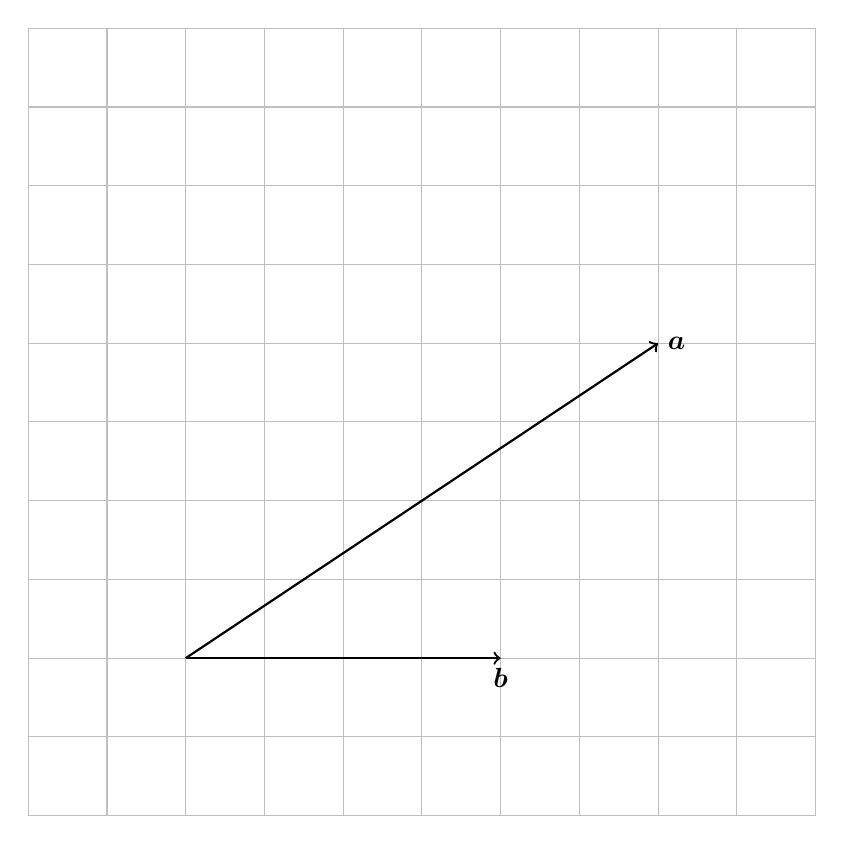
\begin{tikzpicture}[scale=2]
  \draw[thin,step=.5, gray!50] (-1,-1) grid (4,4);
  \draw[->,thick] (0,0) -- (3,2);
    \node[right] at (3,2) {$\bm{a}$};
  \draw[->,thick] (0,0) -- (2,0);
    \node[below] at (2,0) {$\bm{b}$};
\end{tikzpicture}
\end{center}


\begin{enumerate}
  \item Compute the following values and sketch them alongside the vectors \(\ba\) and \(\bb\) above
\begin{enumerate}
    \item \(\mathrm{proj}_{\ba}(\bb)\) and \(\mathrm{orth}_{\ba}(\bb)\)

      \begin{solution}
        \begin{align*}
            \mathrm{proj}_{\ba}(\bb) & = \left(\dfrac{\gen{6,4}\cdot\gen{4,0}}{\gen{6,4}\cdot\gen{6,4}}\right)\gen{6,4}\\
            & = \dfrac{24+0}{36+16}\gen{6,4}\\
            & = \frac{6}{13}\gen{6,4} = \gen{\frac{36}{13},\frac{24}{13}}\\
            \mathrm{orth}_{\ba}(\bb) & = \bb-\mathrm{proj}_{\ba}(\bb)\\
                & = \gen{4,0}-\gen{\frac{36}{13},\frac{24}{13}}\\
                & = \gen{\frac{16}{13},-\frac{24}{13}}
        \end{align*}

        \begin{center}
            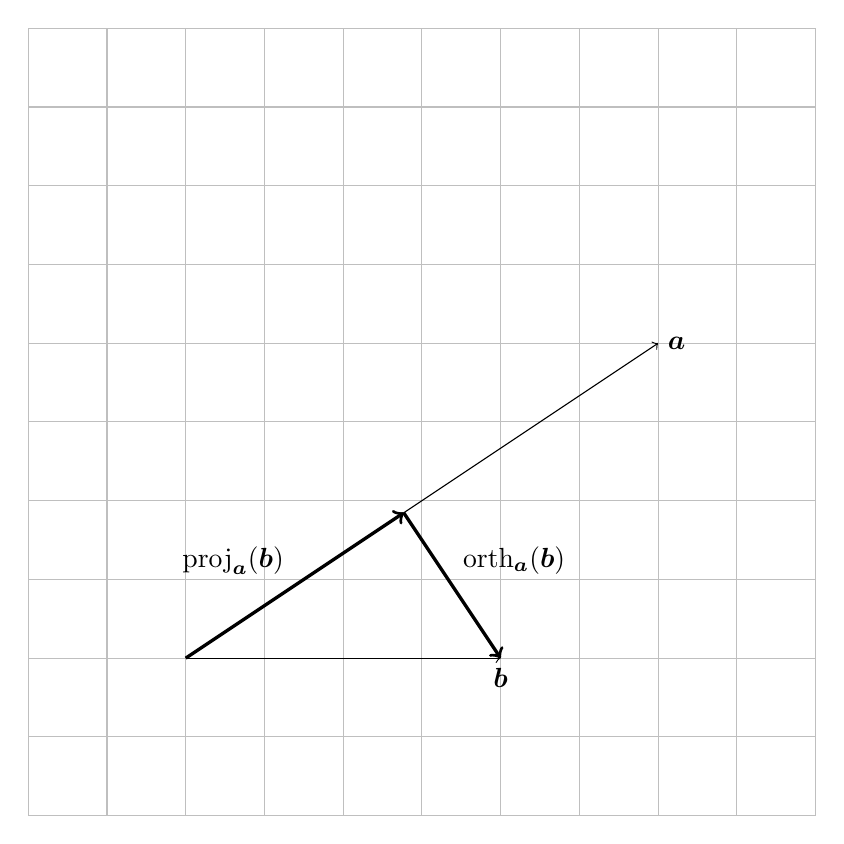
\begin{tikzpicture}[scale=2]
              \draw[thin,step=.5, gray!50] (-1,-1) grid (4,4);
              \draw[->] (0,0) -- (3,2);
                \node[right] at (3,2) {$\bm{a}$};
              \draw[->] (0,0) -- (2,0);
                \node[below] at (2,0) {$\bm{b}$};
              \draw[->,very thick] (0,0)--(36/26,24/26) node[midway,anchor=south east] {$\mathrm{proj}_{\ba}(\bb)$};

              \draw[->,very thick] (36/26,24/26) -- ($(36/26,24/26)+(16/26,-24/26)$) node[midway,anchor=south west] {$\mathrm{orth}_{\ba}(\bb)$};

            \end{tikzpicture}
            \end{center}
      \end{solution}

    \item \(\mathrm{proj}_{\bb}(\ba)\) and \(\mathrm{orth}_{\bb}(\ba)\)

        \begin{solution}
            \begin{align*}          
              \mathrm{proj}_{\bb}(\ba) & = \gen{6,0}
              \mathrm{orth}_{\bb}(\ba) & = \gen{-2,0}
            \end{align*}

            \begin{center}
            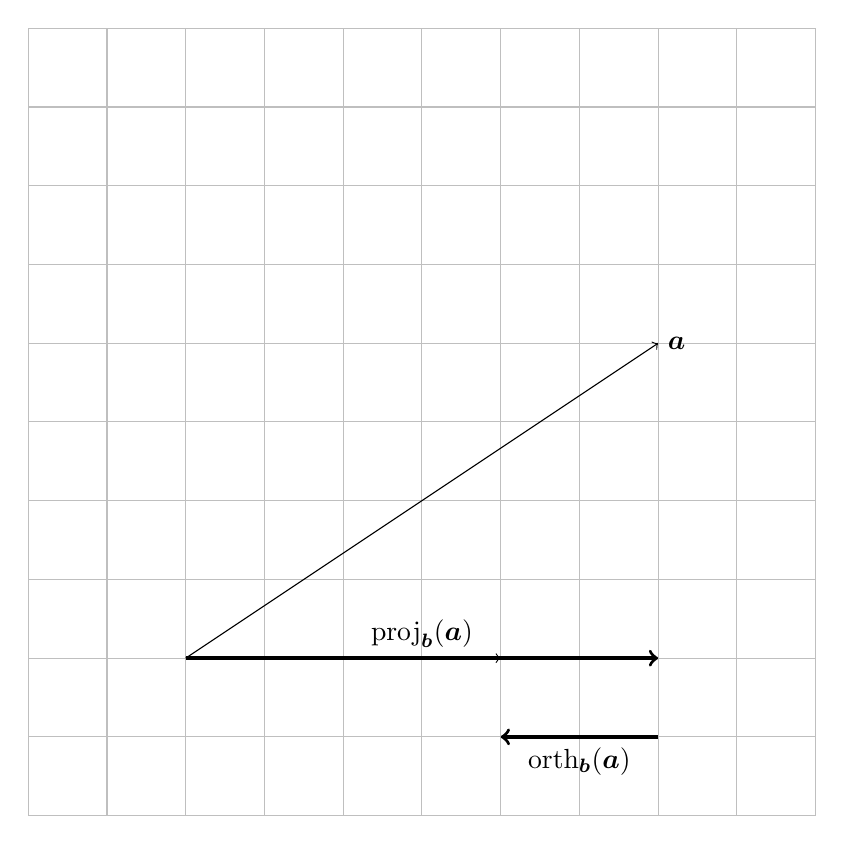
\begin{tikzpicture}[scale=2]
              \draw[thin,step=.5, gray!50] (-1,-1) grid (4,4);
              \draw[->] (0,0) -- (3,2);
                \node[right] at (3,2) {$\bm{a}$};
              \draw[->] (0,0) -- (2,0);
                \node[below] at (2,0) {};

              \draw[->,very thick] (0,0)--(3,0) node[midway,anchor=south] {$\mathrm{proj}_{\bb}(\ba)$};

              \draw[->,very thick] (3,-.5) -- ($(3,-.5)+(-1,0)$) node[midway,anchor=north] {$\mathrm{orth}_{\bb}(\ba)$};

            \end{tikzpicture}
            \end{center}

        \end{solution}
\end{enumerate}
    \item What vector is equal to \(\mathrm{proj}_{\ba}(\bb)+\mathrm{orth}_{\ba}(\bb)\)?

      \begin{solution}
          \(\mathrm{proj}_{\ba}(\bb)+\mathrm{orth}_{\ba}(\bb)\) is always equal to \(\bb\).         
      \end{solution}



    \item Let \(\ba=-5\bm{i}+5\bm{j}+2\bm{k}\) and \(\bb=-\bm{i}+8\bm{j}-\bm{k}\)
    \begin{enumerate}
        \item Compute \(\mathrm{proj_{\ba}(\bb)}\) 
          \begin{solution}
              Using \(\ba=\gen{-5,5,2}\) and \(\bb=\gen{-1,8,-1}\)
              \[
              \mathrm{proj_{\ba}(\bb)}=\left\{-\frac{215}{54},\frac{215}{54},\frac{43}{27}\right\}\approx \{-3.98148,3.98148,1.59259\}
              \]
          \end{solution}
        \item Compute \(\mathrm{orth_{\ba}(\bb)}\)
        \begin{solution}
              \[
                \mathrm{orth_{\ba}(\bb)}=\left\{\frac{161}{54},\frac{217}{54},-\frac{70}{27}\right\}\approx \gen{2.98148, 4.01852, -2.59259}
              \]
              \end{solution}
    \end{enumerate}
\end{enumerate}





%%% Orthogonal projection
\end{document}